\chapter{Représentation du réseau routier}
Un graphe sert mieux à définir l'existence d'une relation entre objets tel qu'une ligne entre deux stations, ce qui est la représentation optimale pour nos données. 

Dans ce chapitre, nous présenterons en première partie les définitions relatives aux graphes et recherche de chemins, ensuite nous passerons à la collecte de données et les différentes approches de représentation prises en compte.
Enfin nous détaillerons la représentation choisie, tout en donnant des exemples.

\section{Généralités sur les graphes}
La théorie des graphes est très probablement née en 1735 lorsque Leonhard Euler (1707 - 1783) résout le problème des sept ponts de Königsberg. 
L'énoncé de ce problème est: la ville de \emph{Königsberg} est une ville autour d'un fleuve, elle compte quatre berges et sept ponts les reliant. Le but du jeu est de savoir s'il existe un chemin permettant d'emprunter tous les ponts une fois et une seule et revenir au point de départ. Le problème s'appelle désormais, de façon plus formelle, la recherche d'un cycle eulérien dans un graphe. Euler a démontré que ce problème n'avait pas de solution.

\begin{figure}[h!]
\center
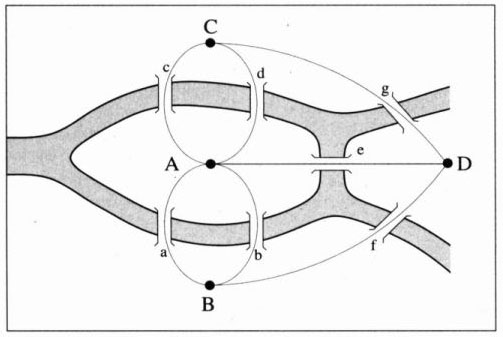
\includegraphics[width=0.75\textwidth]{img/Bridges.jpg}
\caption{Démonstration du problème des septs ponts de Königsberg}
\end{figure}

\subsection{Définitions}
Avant de parler des avantages des graphes, il est important de connaitre la léxique autours de le théorie des graphes \cite{WikiGraphes}.
\begin{description}
\item[Graphe]: un graphe est composé de sommets, et d'arêtes reliant certains de ces sommets.
Un graphe G est défini de manière formelle par un couple (S,A) où :
\begin{itemize}
	\item S est un ensemble fini d'éléments. Chacun de ces éléments est appelé sommet du graphe.
	\item A est un sous-ensemble (éventuellement nul) de SxS. Chacun de ces éléments de A est appelé arête.
\end{itemize}
\item[Arête :] c'est un connexion entre deux sommets A et B. Dans le cas où ce lien est orienté, le terme \textbf{arc} est généralement utilisé.

\item[Poids:] chaque arc/arrête est associé à un poids ou une étiquette qui le décrit. Par exemple, dans un réseau social il peut définir la nature de la relation (ami, famille, collègue) et dans un réseau routier la longueur d'une rue. Parfois le terme \textbf{coût} est utilisé pour décrire le poids.

\item[Successeurs et prédécesseurs:] dans un arc (x, y) d'un graphe, le sommet \emph{y} est appelé \textbf{successeur} de \emph{x} et \emph{x} est dit \textbf{prédécesseur} de \emph{y}.\newline
les sommets \emph{x} et \emph{y} sont des sommets voisins (ou adjacents).

\item[Graphe connexe] : un graphe est connexe si on peut atteindre n'importe quel sommet à partir d'un sommet quelconque en parcourant différentes arêtes/arcs.

\item[Graphe directionnel] : aussi appelé graphe orienté, digraphe ou un réseau dirigé, c'est un graphe où tous les sommets sont reliés par des arcs.
Un graphe où les sommets sont reliés par des arêtes est appelé un graphe non-orienté

\item[Chemin] : un chemin est une suite finie et consécutive de sommets et d'arcs, ou d'arcs uniquement, débutant et finissant par un sommet source et un sommet destination, tel que chaque arc sortant d'un sommet est incident (entrant) au sommet suivant dans cette séquence.
La figure \ref{fig:chemin} donne un exemple d'un chemin orienté.
\begin{figure}[h]
	\centering
	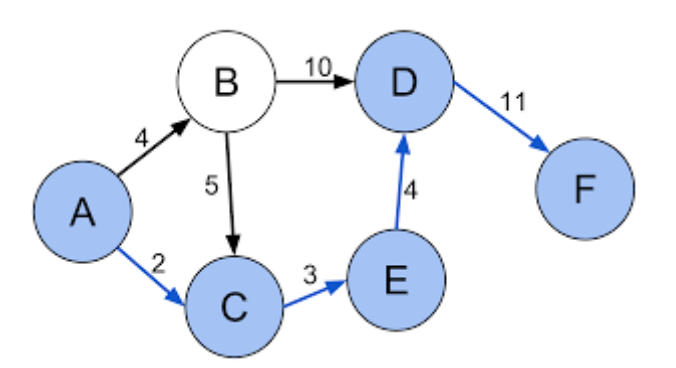
\includegraphics[width=0.55\textwidth]{img/cheminGraphe.png}
	\caption{Exemple de chemin orienté}
	\label{fig:chemin}
\end{figure}
\end{description}

	
	
\section{Avantages d'utilisation d'un graphe}
\subsection{Domaines d'utilisation des graphes}
Un graphe sert avant tout à manipuler des concepts, et à établir un lien entre ces concepts. N'importe quel problème comportant des objets avec des relations entre ces objets peut être modélisé par un graphe.
Les graphes sont donc des outils très puissants et largement répandus qui se prêtent bien à la résolution de nombreux problèmes. Voici quelques-uns :

\begin{description}


\item[Recherche de chemin (PathFinding)]
Un cas très fréquent. Chaque nœud représente une position et chaque arête est un chemin entre deux positions, ou en remplaçant les nœuds par des adresses et les arêtes par des routes, on obtient le graphe utilisé par les GPS ou les outils de cartographie tel que Google Map.
La recherche de chemins est aussi utilisée en biologie, communications (réseaux de télécommunications)...etc.
Il est courant de chercher le chemin le plus court entre deux positions dans la plupart de ces domaines, nous nous intéressons particulièrement à ce cas d'utilisation, que nous discuterons en détail dans la section suivante.


\item[L'ordonnancement de tâches:]
On peut représenter chacune des tâches à effectuer par un nœud, et les dépendances entre chacune de ces tâches par des arcs.
On cite l'exemple de l'ordonnancement des projets, les graphes permettent de planifier les différentes tâches d'un projet, détecter les tâches pouvant être effectuées simultanément et estimer la durée totale du projet.

\item[Les systèmes de recommandation:]
C'est une forme spécifique de filtrage de l'information qui a pour but de présenter à un utilisateur des éléments qui sont susceptibles de l'intéresser, en se basant sur ses préférences et son comportement.
Les moteurs de recommandation font usage des graphes pour représenter des individus ou objets et leurs différents liens. Cet outil est très utilisé en sciences sociales, par exemple le graphe social de Facebook qui représente les associations entre des personnes ou le réseau LinkedIn qui est un graphe de relations entre des professionnels...etc.

Le but est de pouvoir identifier les communautés formées, les centres d'intérêts communs, en suggérant à l'utilisateur les choses qu'il est susceptible d'aimer, les personnes qu'il connaît peut-être, et avant tout (et surtout) pour créer des publicités ciblées adaptées à chacun.

\end{description}

\section{Recherche de Chemin:}

\subsection{Définition:}
La recherche du plus court chemin est la capacité pour un système de déduire le chemin approprié autour des obstacles pour atteindre un point de destination tout en évitant les obstacles et en parcourant la distance la plus petite possible.
Le choix de la méthode de l'analyse et sa complexité peuvent augmenter à mesure que d'autres circonstances doivent être analysées, en prenant en compte différentes contraintes :

\begin{itemize}
	\item \textbf{Poids:} certains algorithmes n'acceptent que des arcs dont le poids est positif.
	\item \textbf{Type d'algorithme:} il existe des algorithmes qui calculent le plus court chemin de nœud à nœud, entre toutes les paires de nœuds ou encore d'un nœud vers tous les autres.
	\item \textbf{Prise en compte d'informations externes:} l'utilisation d'une connaissance externe à la structure du graphe peut parfois accélérer la recherche.
\end{itemize}

\subsection{Domaines d'utilisation :}
Le problème du plus court chemin est parmi les problèmes les plus étudiés de la théorie des graphes, on le retrouve dans beaucoup de domaines :
\begin{itemize}
\item\textbf{Optimisation des réseaux:} réseaux routiers, de télécommunications, de distribution.
\item\textbf{Réseaux informatiques et protocoles de routage: } les protocoles de routages permettant de trouver les meilleurs chemins pour passer les paquets réseaux utilisent ces algorithmes, tel que le protocole OSPF (Open Shortest Path First).
\item\textbf{Biologie:} il est utilisé pour étudier la propagation d'une maladie infectieuse, par exemple.
\item\textbf{Cartographie:} pour mesurer le chemin le plus court entre deux lieux ou villes.
\end{itemize}

\subsection{Les algorithmes de recherche de chemin}
Les algorithmes de calcul d'itinéraires origine-destination(s) sont des algorithmes qui permettent de calculer le plus court chemin d'un sommet source vers tous les autres sommets avec une complexité polynomiale.\newline
 On les répartit classiquement en deux familles : 
\begin{itemize}
	\item \textbf{A fixation d'étiquette} (Label setting algorithms): Ce type d'algorithme choisissent à chaque itération un sommet x, et calculent sa valeur définitive V[x]. Cette valeur V[x], appelée étiquette, sert à définir la valeur du plus court chemin vers le sommet x.
	L'avantage principal de ces algorithmes est qu'il est possible d'arrêter la recherche de chemin dès atteinte du nœud destination puisque son étiquette sera fixée définitivement.
	L'algorithme à correction d'étiquette le plus célèbre est l'algorithme de \textbf{Djikstra}.
	
	\item \textbf{A correction d'étiquette} (Label correcting algorithms): Ces algorithmes peuvent affiner et corriger les étiquettes de chaque sommet jusqu'à la dernière itération.
	Ils ne sont pas forcément moins performants que les algorithmes à fixation d'étiquette, et ont une utilisation plus générale, lors de présence de poids négatives dans le graphe où l'algorithme de Djikstra, par exemple, n'est pas utilisable.\newline
	Un exemple bien connu est l'algorithme de \textbf{Bellman-Ford}.
\end{itemize}

Malgré leur complexité polynomiale, ces algorithmes peuvent engendrer des temps de calculs importants pour des graphes de grande taille, ce qui a suscité le développement des techniques d'accélération (visant souvent l'optimalité plutôt qu'un meilleur chemin) comme l'algorithme A* qui est le plus célèbre, le parcours en largeur/profondeur, le parcours bidirectionnel, ainsi que les méthodes de pré-traitement (pré-calculer les meilleurs chemins dans tout les nœuds par exemple).

Dans notre cas, et vu que le graphe de la première version est statique (ne changera pas après avoir calculé le chemin), le choix le plus pertinent serait l'\textbf{algorithme A*}.
Cependant, ce dernier nécessite une fonction heuristique\FancyFootNote{Heuristique: une méthode de calcul qui fournit rapidement une solution réalisable, pas nécessairement optimale ou exacte, pour un problème d'optimisation difficile.} pour estimer le meilleur nœud suivant, ce qui sera difficile à concevoir sans une bonne connaissance de notre problème et dans les limites du temps de ce projet.
De ce fait, nous avons opté pour une approche plus simple utilisant l'algorithme BFS qui est simple à implémenter et à adapter à nos besoins, pour ainsi avoir rapidement une version minimale de l'application, cet algorithme sera présenté dans la section suivante.\newline
Nous avons pris en compte la possibilité de changer l'algorithme de recherche dans de futures version de l'application, en prenant une structure plus flexible qui sera expliquée dans le chapitre suivant.

\subsection{L'algorithme BFS (Breadth-First-Search)}

\begin{enumerate}
	\item \textbf{Présentation}: BFS\cite{refBFS} est un algorithme de parcours ou de recherche dans un arbre ou graphe, il commence d'un nœud source (ou la racine de l'arbre) et explore ses nœuds successeurs d'abord, 

Cet algorithme est très similaire au parcours par largeur d'un arbre, sauf qu'un graphe peut avoir des cycles, donc pour éviter de recalculer le même nœud deux fois, il garde une liste de nœuds visités.

	\item \textbf{Complexité:} la complexité temporelle de l'algorithme est de O(V+E), où V est le nombre de sommets et E le nombre d'arcs.
	
	\item \textbf{Étapes de l'algorithme:}
		L'algorithme effectue un parcours en largeur sur le graphe, en d'autres mot un parcours par niveau, il traite tous les nœuds voisins du nœud de départ avant de passer aux nœuds voisins des nœuds visités.
\begin{figure}
	\center
	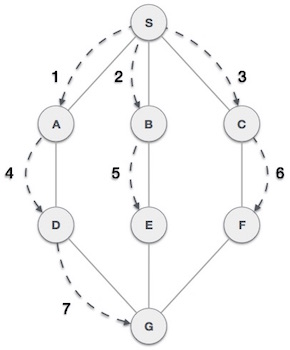
\includegraphics[scale=0.6]{img/BFS.jpg}
	\caption{Déroulement d'un parcours BFS.}
\end{figure}		
L'algorithme utilise une file pour mémoriser les nœuds suivants à visiter, les étapes de l'algorithme se résument en les règles suivantes:
	\begin{enumerate}
		\item Visiter le nœud suivant non visité du nœud courant, le marquer comme visité, traiter le nœud et l'insérer dans la file.
		\item Si aucun autre nœud voisin n'est trouvé, retirer le premier nœud de la file.
		\item Répéter les étapes (a) et (b) jusqu'à ce que la file soit vide.
	\end{enumerate}
	Le BFS traverse donc seulement les nœuds qui peuvent être atteints depuis le nœud de départ.
\end{enumerate}

\section{Collecte de données}
Afin de mieux tester notre application, nous avons tenté de collecter un maximum de données réelles, à commencer par contacter l'Entreprise de Transport d'Oran, puis ensuite traiter ces informations et ajouter d'autres que nous avons collectés par nous-mêmes.
Le résultat de cette collecte est comme suit :

\subsection{ETO (Entreprise de Transport d'Oran)}

%what they did gave u
Nous avons été bien accueillis par l'un des responsables de l'ETO que nous remercions de nous avoir bien expliqué le fonctionnement des lignes de notre région ainsi que d'avoir fourni plusieurs informations utiles, tel que:
\begin{itemize}
	\item La liste des lignes et leur longueur totale.
	\item Les différents horaires de travail (été/hiver/fin de semaine...etc).
	\item La fréquence des bus et les différentes contraintes spécifiques à notre région, comme le manque de calendrier d'horaires qui décrivent le temps de passage de chaque bus.
	\item Le nombre de bus desservant chaque ligne.
	\item Le nom de chaque station.
\end{itemize}

% but that wasnt enough
En plus du catalogue que nous avons reçu, leurs informations nous ont permis de bien tracer les spécifications et les particularités de ces lignes.
Cependant, ces informations n'ont pas été suffisantes pour notre travail, en effet:
	\begin{itemize}
	\item Nous avions besoin de noms plus significatifs pour chaque station, car les noms fournis étaient des noms communs connues par les habitants seulement.
	\item Le catalogue ne contenant pas les adresses exacte ou les coordonnées de chaque station.
	\item Pas d'informations sur la distance entre chaque station.
	\end{itemize}
	
%thx again for trying
Nous remercions encore l'ETO pour leur assistance, néanmoins ces données doivent être traitées davantage, réorganisées et complétées avant qu'elles puissent être intégrées dans notre application.

\begin{figure}
	\center
	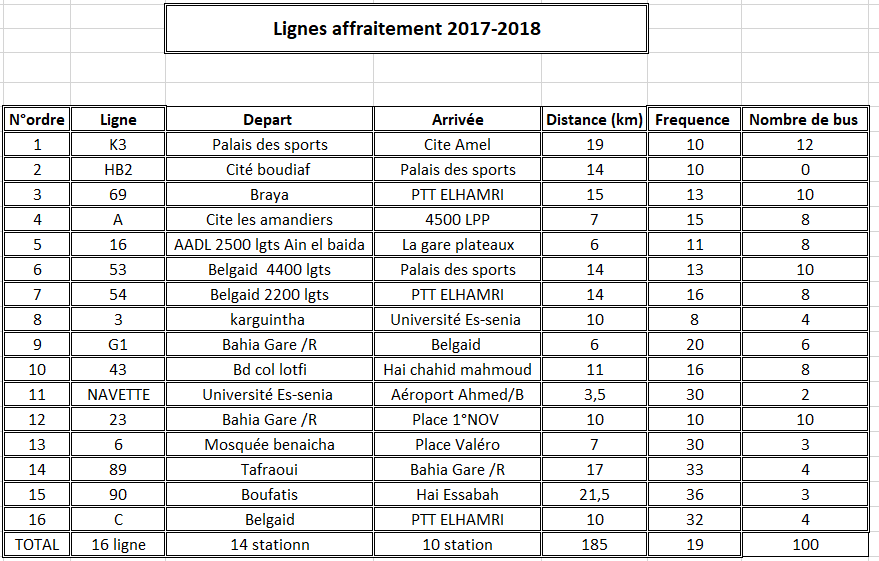
\includegraphics[scale=0.7]{img/LignesETO.png}
	\caption{Échantillon de données reçues par l'ETO.}
\end{figure}

\subsection{Données supplémentaire}
	\begin{itemize}
		\item Malgré l'absence de données officielles, nous avons réussi à trouver sur le net différentes sources supplémentaires pouvant nous aider pour compléter nos données : notamment des listes de différents lieux de la ville d'Oran contenant des noms complets et des adresses permettant de compléter les données de l'ETO.
		\item Le site officiel de la Setram (Société d'Exploitation des Tramways) a été suffisant pour récupérer toutes les données concernant la ligne du Tramway, ses horaires et même les temps d'attente pour chaque arrêt.
		\item Pour assurer l'intégrité des données et leurs mise à jour constantes, une des solutions proposées est d'ajouter une fonctionnalité permettant à des utilisateurs ou à une autorité de signaler un changement de lignes, une estimation de temps trop imprécise ou suggérer des chemins que l'application n'a pas calculé, ceci permettra de faire fonctionner et évoluer cette application à l'aide de \emph{crowdsourcing}\FancyFootNote{crowdsourcing: ou production participative, c'est l'utilisation de connaissance d'un grand nombre de personnes comme une communauté d'internautes ou des utilisateurs d'un produit, pour réaliser une tâche traditionnellement faite par des employés.} seulement.
	\end{itemize}

\subsection{Traitement de données}
Les données obtenues de l'ETO et de l'Internet ont permis de rassembler les informations suivantes :
\begin{itemize}
	\item Différentes informations sur le fonctionnement de lignes.
	\item Liste des lignes de bus publiques et les stations desservies, les noms des stations étant toujours pas claires et sans adresses.
	\item Longueur totale de chaque ligne, fréquence et nombre de bus de chaque ligne.\newline 
\end{itemize}

Depuis ces informations nous avons déduit d'autres informations utiles, notamment :

\begin{itemize}
	\item \textbf{Temps d'attente : } Les bus n'ayant pas de calendrier précis, nous avons utilisé la distance totale, fréquence et nombre de bus pour déduire approximativement le temps d'attente dans chaque arrêt entre deux bus.
	\item \textbf{Coordonnées GPS :} Afin d'afficher les stations sur une carte, les coordonnées GPS, ou au moins des adresses précises permettant de générer les coordonnées avec un outil de cartographie, sont nécessaires. Cependant, les données que nous avons ne sont pas suffisantes. 
	Ainsi, pour mieux introduire les lignes et stations dans l'application, il a été nécessaire d'implémenter une fonctionnalité dans l'application administrateur qui permettrait de marquer les stations sur une carte et enregistrer les informations nécessaires automatiquement. L'aperçu de cette interface est donné dans la section \ref{ref:Implementation}.
\end{itemize}

	
\section{Construction du graphe}
Après avoir présenté quelques généralités sur graphe, et détaillé les données que nous avons collecté, nous passons aux différents détails sur comment est construit notre graphe et comment le stocker.
\subsection{Différentes approches pour stocker le graphe}
\begin{itemize}
	\item \textbf{Outils Open Source (OpenTripPlanner)} : 
	      Il existe plusieurs outils qui proposent ce service, en particulier OpenTripPlanner : un projet Open Source qui permet de créer un réseau routier à partir de données GTFS \FancyFootNote{GTFS (General Transit Feed Specification ou spécification générale pour les flux relatifs aux transports en commun) : est un format informatique standardisé pour communiquer des horaires de transports en commun et les informations géographiques associées.}, ces données seront ensuite intégrées avec OpenStreetMap et stockées sur le serveur, qui exposera une API REST pour questionner le serveur : recherche de Chemin, possibilité d'intégrer les horaires, ...etc.
	      		
	      Vu la nature un peu particulière du réseau d'Oran, et la non-disponibilité des données (Données officielles des lignes et données (adresses) sur OpenStreetMap), cette solution ne sera pas envisagée. 
	      Cependant, l'application prendra une architecture flexible permettant d'intégrer, au futur, de tels outils rapidement si une solution est possible.
	\item \textbf{Représentation indépendante de chaque ligne en tables SQL}
	      Une des approches considérées était de représenter chaque ligne indépendamment, l'algorithme du service aura à chercher des points de liaison entre ces lignes.
	      L'avantage principal de cette approche est la facilité de manipulation de ces données de lignes, en ajoutant/supprimant des lignes sans conflit.
	      Cette approche présente par contre un inconvénient majeur au niveau des performances, vu que l'utilisation d'un algorithme de PathFinding requiert l'utilisation de plusieurs tables (lignes) à chaque requête.
	      
	\item \textbf{Utiliser une base de données orientée graphe}: nous avons finalement choisi d'utiliser une base de données orientée graphe qui permet de stocker en permanence le graphe, mais aussi de fournir plusieurs opérations pour créer des nœuds et des relations, les modifier et les parcourir pour rechercher des chemins ou effectuer certains calculs.
	
Comparé au stockage par tables SQL, cette approche offre un accès plus rapide et simple en parcourant un graphe déjà construit tout en tirant les meilleures performances des différents algorithmes de recherche de chemins.

	Nous avons, cependant, noté certaines difficultés suivant cette représentation, notamment dans la modification ou suppression de lignes où le changement ou la suppression d'une seule station peut affecter plusieurs autres lignes.\newline
	Ainsi, comme l'ajout d'une station au milieu d'une ligne impliquera la suppression de plusieurs arcs, nous avons décidé, comme première solution, de restreindre les modifications et suppressions de nœuds aux stations qui ne sont reliées à aucune ligne, et pour les lignes, de supprimer toute la ligne et reconstruire les arcs à chaque modification.
	     
\end{itemize}
\subsection{Représentation choisie du graphe}
La figure \ref{fig:structGraph} présente la structure utilisée pour représenter toutes nos données dans le graphe:
\begin{itemize}
	\item Chaque nœud avec l'étiquette \emph{:Station} représenterait une station de transport quelconque.
	\item Chaque arc entre stations représente le passage d'un transport public entre ces deux stations, ces arcs sont étiquetés par le type du transport (Bus, Tramway,..etc.), chaque type contient les différentes données de chaque transport comme le nom du Bus.
\end{itemize}

\begin{figure}[h!]
	\center
	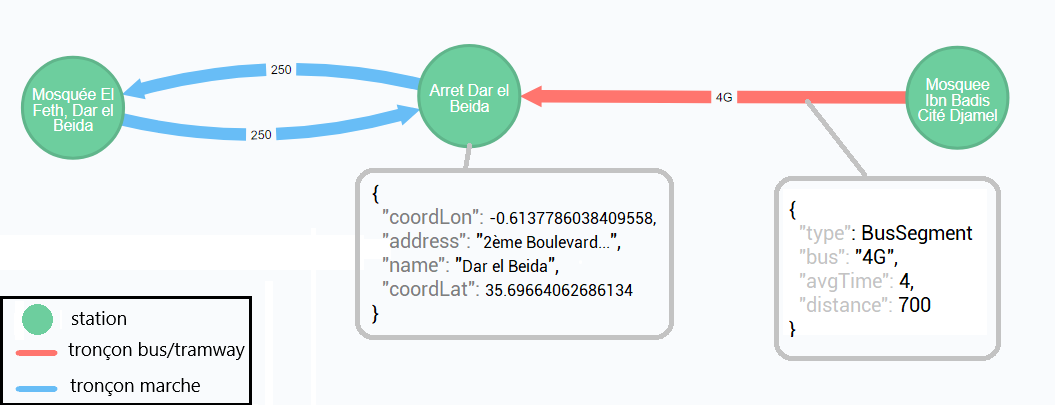
\includegraphics[width=\textwidth]{img/structureGraphe.png}
	\caption{Représentation en graphe du réseau routier}
	\label{fig:structGraph}
\end{figure}

\begin{figure}[h!]
	\center
	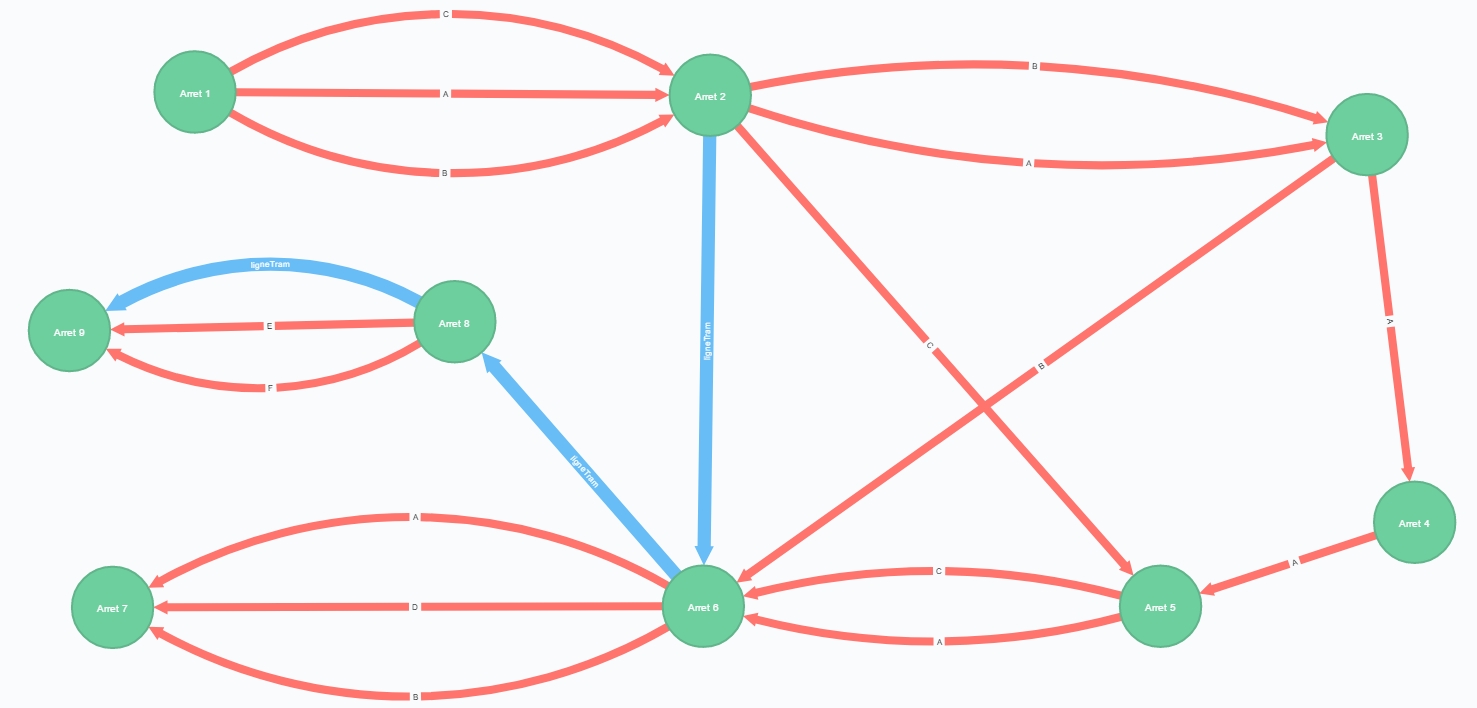
\includegraphics[width=1.1\textwidth]{img/GrapheNeo4j.png}
	\caption{Aperçu d'un graphe de transport}
\end{figure}

\textbf{Arcs de bus: } Chaque arc contient uniquement l'identifiant du Bus qui le concerne, les autres informations de chaque bus (temps d'arrêt, prix...etc.) peuvent être représentés séparément comme d'autres nœuds étiquetés dans le graphe ou stockés ailleurs dans une base de données différente. \newline
Nous avons choisi de ne garder que les données les plus importantes dans cette première version, nous pouvons ajouter d'autres propriétés et informations dans le graphe au fur et à mesure que l'application évolue.

%
%	\begin{itemize}
%		 \item Arcs étiquetés par le type du transport ( BusSegment, TramSegment, WalkSegment. ..) 
%		 \item Représenter chaque bus séparément ( pour faciliter la recherche et filtre ) 
%		 \item Nœuds (Stations) ont les attributs suivants : 
%		 \begin{itemize}
%		 	\item Nom.
%		 	\item Adresse.
%		 	\item Tableau de coordonnées (pour chaque direction) avec indicateur de direction.
%		 \end{itemize}
%		 \item Arcs ont les attributs suivants :
%		 \begin{itemize}
%		 		\item Dist : distance entre les deux stations
%		 		\item Time: temps moyen pour passer de la première station à la deuxieme
%		 		\item Bus : ( pour les arcs de type Bus ) nom/id du bus.
%		 		** remarque : infos du bus ( temps d'arrêt, prix ..etc) sont stockés sépareraient.
%		 \end{itemize}
%	\end{itemize}

\subsection{Cas de la marche}
Afin de pouvoir intégrer la marche dans la recherche de chemin, il est nécessaire de pouvoir détecter les arrêts les plus proches de chaque arrêt pendant le traitement, et essayer de considérer les arrêts les plus proches de chaque nœud visité.\newline 
Cette solution s'avère difficile à appliquer dans la version actuelle du projet, nous avons donc choisi de représenter la possibilité de marcher avec un arc similaire aux arcs de transports.\newline
Ces arcs sont automatiquement ajoutés à la création de chaque ligne en calculant toutes les distances entre le début et fin de la ligne ajoutée avec le début et fin de chaque autre ligne, et ajouter un arc dans les deux sens si la distance est inférieur à 1Km (valeur arbitraire).
Un exemple de cet arc est donné dans la figure \ref{fig:structGraph}.

Cette approche permet d'intégrer la marche de façon minimale sans affecter les performances et sans avoir à calculer des distances pendant la recherche du chemin.
Il sera possible d'améliorer cette fonctionnalité après avoir implémenté la recherche des plus proches stations directement dans le graphe à partir d'un point donné, sans avoir à comparer toutes les stations (voir chapitre des perspectives).

\section{Conclusion}
Nous avons, dans ce chapitre, présenté les différentes généralités sur les graphes et données collectés ainsi que comment est construit notre graphe pour ce projet.
Malgré les différentes contraintes (complexité du problème, manque de données, spécificités des lignes d'Oran), la représentation choisie pour cette première version reste suffisante et facilement extensible pour de futures améliorations.
\newpage
